\documentclass[10pt,twocolumn,letterpaper]{article}

\usepackage{cvpr}
\usepackage{times}
\usepackage{epsfig}
\usepackage{graphicx}
\usepackage{amsmath}
\usepackage{amssymb}
\usepackage{multirow}

\graphicspath{ {./images/} }

% Include other packages here, before hyperref.

% If you comment hyperref and then uncomment it, you should delete
% egpaper.aux before re-running latex.  (Or just hit 'q' on the first latex
% run, let it finish, and you should be clear).
\usepackage[breaklinks=true,bookmarks=false]{hyperref}

\cvprfinalcopy % *** Uncomment this line for the final submission

\def\cvprPaperID{****} % *** Enter the CVPR Paper ID here
\def\httilde{\mbox{\tt\raisebox{-.5ex}{\symbol{126}}}}

% Pages are numbered in submission mode, and unnumbered in camera-ready
%\ifcvprfinal\pagestyle{empty}\fi
\setcounter{page}{1}
\begin{document}

%%%%%%%%% TITLE
\title{Fuzzy Rules for Segmentation of Remotely Sensed Images}

\author{Andrea Montemurro\\
Universitá degli Studi di Bari "Aldo Moro"\\
{\tt\small a.montemurro23@studenti.uniba.it}
% For a paper whose authors are all at the same institution,
% omit the following lines up until the closing ``}''.
% Additional authors and addresses can be added with ``\and'',
% just like the second author.
% To save space, use either the email address or home page, not both

}

\maketitle
%\thispagestyle{empty}

%%%%%%%%% ABSTRACT
\begin{abstract}
Segmentation of remotely sensed images is a complicated task because the images do not depict well-defined objects.
To overcome this problem, fuzzy logic is really useful as it allows to classify these objects with a degree of uncertainty.

This work analyzes the use of an Adaptive Neuro Fuzzy Inference System (ANFIS) for the production of Fuzzy Rules that classify the pixels of remotely sensed images, for the semantic segmentation of this type of images.

This system guarantees a good level of accuracy in the pixel classification despite the few input features and, unlike the classic deep learning techniques, is also explanatory since the classification rules it produces are similar to the way of thinking of human beings.
\end{abstract}

%%%%%%%%% BODY TEXT
\section{Introduction}

In computer vision image segmentation is the process of partitioning a digital image into multiple segments (sets of pixels, also known as image objects). The goal of segmentation is to simplify and/or change the representation of an image into something that is more meaningful and easier to analyze. Image segmentation is typically used to locate objects and boundaries in images. More precisely, image segmentation is the process of assigning a label to every pixel in an image such that pixels with the same label share certain characteristics.~\cite{segmentation} The result of image segmentation is a set of segments that collectively cover the entire image, or a set of contours extracted from the image. Each of the pixels in a region are similar with respect to some characteristic or computed property, such as color, intensity, or texture.

Remote sensing images cover diversified applications in meteorology, agriculture, geology, biodiversity conservation, land use planning, education, intelligence, warfare. The images can be acquired in color in the visible spectrum (for example in the RGB spectral bands) or in other electromagnetic spectra (for example in the infrared). The semantic segmentation of this type of images is an important task to make them usable and also understandable by human beings, in the fields of application mentioned above. A typical problem with this type of image is that the objects are not clearly defined and / or separated from each other.

Numerous approaches especially based on deep learning and on the use of neural networks have been proposed in the literature. Fuzzy logic was also successfully applied to solve this task.
The aim of this work is to analyze the use of a system based on both of these two approaches in a hybrid manner. Considering the satellite imagery problem mentioned above, fuzzy logic has the advantage of being able to classify the classes/objects of the photos with a certain degree of uncertainty. Furthermore, fuzzy logic approaches have the advantage of being more explanatory than others, for example those based on the use of Artificial Neural Networks (ANNs)~\cite{QiuJenenr}.

F.Qiu and J. R. Jensen~\cite{QiuJenenr} have already demonstrated the efficacy of ANFIS in the segmentation of multi spectral remotely sensed images, but in this work only RGB images were used, as they are more easily available in a free way and easier to process.

%-------------------------------------------------------------------------
\subsection{Related Work}

With breakthroughs in the computational power of graphic processing units (GPUs) and the development of big data, considerable progress in deep convolutional neural networks has occurred in recent years. Semantic segmentation is a successful application of this approach and has been utilized to solve pixel-wise classification problems.

Neurons with nonlinear activation functions are arranged in layers and act like a set of piece-wise nonlinear simulators~\cite{neurApproximators}. Neural networks are able to learn from existing examples adaptively, which makes the classification objective~\cite{classificationObjective}. At the same time, various noise information inevitably included in the examples supply a trained neural network with the ability to generalize, which makes neural networks robust solutions in the presence of previously unseen, incomplete or imprecise data~\cite{impreciseData}.
 Long et al.~\cite{long} proposed a semantic segmentation technique that replaced the fully connected layers with convolutional layers to enable end-to-end training, and utilized deconvolution~\cite{deconvolutional} layers to predict high-resolution masks from coarse feature maps. In addition, to strengthen the segmentation performance, skip connections between pooling~\cite{gradientBased} layers were used to fuse the semantic features and appearance features (FCN-8s, FCN-16s and FCN-32s) obtained by the network. The FCNs combined the features from the final three layers (FCN-8s), which made it similar to an incomplete encoder-decoder structure. UNet~\cite{unet} used a symmetric and complete encoder-decoder structure for image segmentation, including a contracting path and a similar expanding path in which the pooling layers were replaced by upsampling layers. For precise location, high-resolution features from each layer in the contracting path were combined with upsampled outputs from the corresponding expanding path through a long skip connection. This elegant architecture yielded outstanding performance with very few images. SegNet~\cite{segnet}, which was proposed by Vijay et al., officially showed a typical deep convolutional encoder-decoder structure. The encoder was responsible for object classification, and the corresponding decoder reconstructed the encoding features to the same size as the original input. In particular, the decoder used the pooling indices memorized from the corresponding encoder to perform upsampling, which produced a sparse feature map and could be trained effectively. The encoder-decoder structure is the most popular structure for semantic segmentation.
 
Despite the excellent performance of neural networks in image segmentation, it is difficult to provide a comprehensible explanation of the process through which a given output has been obtained from a neural network~\cite{critique}. Therefore, a neural network is often accused of being a black box, which hides the relation between inputs and outputs in the weights of the neurons of its "hidden" layers. As a result, is difficult to gain any understanding of the problem at hand due to the lack of an explanatory capability to provide insight into the characteristics of the dataset. For the same reason, it is also difficult to incorporate human expertise to simplify, accelerate or improve the performance of image classification, in fact, a neural network often has to learn from scratch~\cite{dataManual}.
On the other hand, it is possible to represent image (pixel) classification decision explicitly in the form of declarative fuzzy "if-then" rules. Fuzzy systems are an extension of traditional expert systems.
Therefore, if these two approaches (Fuzzy systems and neural networks) are combined, one technology can provide the capabilities not available in the other. The integration of neural networks and fuzzy systems is often known as neuro-fuzzy systems in artificial intelligence~\cite{dataManual}.

%-------------------------------------------------------------------------
\section{Methods}

In this work, the ANFIS proposed by Jang~\cite{jang} is used, which assumes a Takagi Sugeno Kang (TSK) style of defuzzification rather than the more usual Mamdani style.

%-------------------------------------------------------------------------
\subsection{Fuzzy If-Then Rules}

Fuzzy  if-then rules or fuzzy conditional statements are expressions of the form IF A THEN B, where A and B are labels of fuzzy sets characterized by appropriate  membership functions. Due  to their  concise  form, fuzzy if-then rules are often employed to capture the imprecise modes of reasoning that play an essential role in the human ability to  make decisions in an environment of uncertainty and imprecision.~\cite{jang} 

%-------------------------------------------------------------------------
\subsection{Fuzzy Inference System}

\begin{figure}[h]
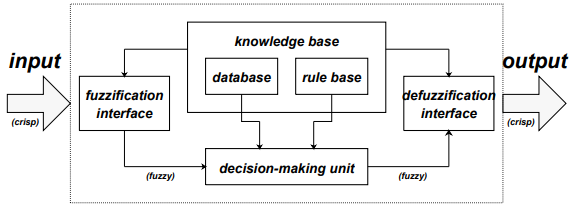
\includegraphics[width=8cm]{images/inferenceSys.PNG}
\caption{A fuzzy inference system}
\end{figure}
Basically a fuzzy  inference system  is composed  of five functional blocks:
\begin{enumerate}
    \item a rule base containing a number of fuzzy if-then rules;
    \item a database which defines the membership functions of the fuzzy sets used in the fuzzy rules;
    \item a decision-making unit which performs the inference operations on the rules;
    \item a fuzzification interface which transforms the crisp inputs into degrees of match with linguistic values;
    \item a defuzzification interface which transform the fuzzy results of the inference into a crisp output.~\cite{jang}
\end{enumerate}
The steps of fuzzy reasoning (inference operations upon fuzzy if-then rules) performed by fuzzy inference systems are:
\begin{enumerate}
    \item  Compare the input variables with the membership functions on the premise part to obtain the membership values (or compatibility measures) of each linguistic label. (This step is often called fuzzification).
    \item Combine (through a specific T-norm operator, usually multiplication or min.) the membership values on the
premise part to get firing strength (weight) of each rule.
    \item Generate the qualified consequent (either fuzzy or crisp) of each rule depending on the firing strength
    \item Aggregate the qualified consequents to produce a crisp output. (This step is called defuzzification).~\cite{jang}
\end{enumerate}

\begin{figure}[h]
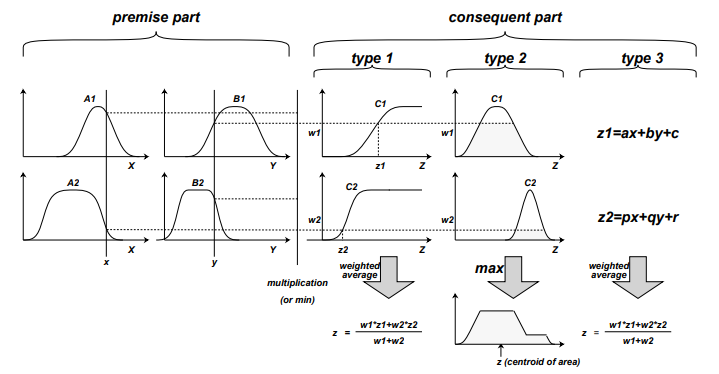
\includegraphics[width=8cm]{images/commonUsed.PNG}
\caption{Commonly used fuzzy if-then rules and fuzzy reasoning mechanisms~\cite{jang} }
\end{figure}
Depending on the types of fuzzy reasoning and fuzzy if-then rules employed, most fuzzy inference systems can be classified into three types~\cite{jang}, as shown in the previous figure. The model used in this work uses a type 2 system, in which the overall fuzzy output is derived by applying “max” operation to the qualified fuzzy outputs (each of which is equal to the minimum of firing strength and the output membership function of each rule)~\cite{jang}.

%-------------------------------------------------------------------------
\subsection{Adaptive Networks}

\begin{figure}[h]
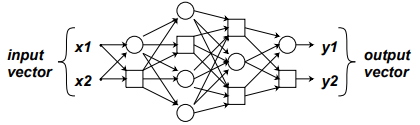
\includegraphics[width=8cm]{images/adaptiveNet.PNG}
\caption{An adaptive network.}
\end{figure}
An adaptive network is a  is a multi-layer feedforward neural networks with supervised learning capability. An adaptive network in which each node performs a particular function (node function) on incoming signals (in the particular case of this work they are the values of the three colors of each pixel and the entropy value) as well as a set of parameters pertaining to this node. Moreover, part or all of the nodes are adaptive, which means each output of these nodes depends on the parameter(s) pertaining to this node, and the learning rule specifies how these parameters should be changed to minimize a prescribed error measure~\cite{jang}.

The ANFIS implementation used in this work uses a batch (off-line) learning that use an hybrid learning rule which combines the gradient method and the least squares estimate (LSE) to identify parameters.~\cite{jang}.

%-------------------------------------------------------------------------
\subsection{ANFIS architecture}

\begin{figure}[h]
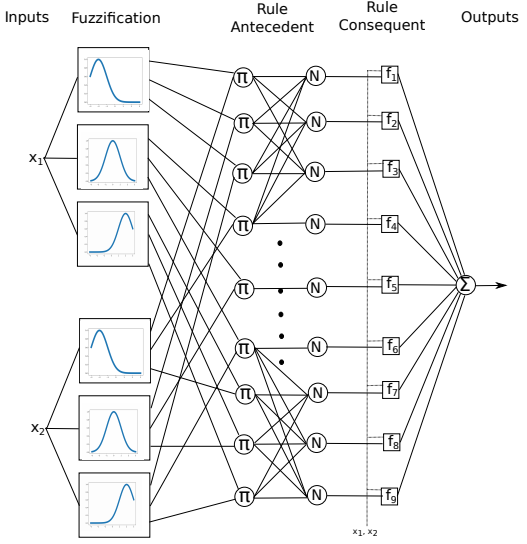
\includegraphics[width=8cm]{images/anfis-layers.PNG}
\caption{The ANFIS structure.}
\end{figure}
In the \textbf{layer 1} every node $i$ is a square node with a node function
\begin{equation}
O_{i}^{1}=\mu_{A_{i}}(x)
\end{equation}
where $x$ is the input to node $i$, and $A_{i}$ is the linguistic label associated with this node function.$O_{i}^{1}$ is the membership function of $A_{i}$ and it specifies the degree to which the given $x$ satisfies the quantifier $A_{i} .$ In this work, a Gaussian $\mu_{A_{i}}(x)$ function is used, but other membership functions can be used.
$$
\mu_{A_{i}}(x)=\exp \left[-\left(\frac{x-c_{i}}{a_{i}}\right)^{2}\right]
$$
where $\left\{a_{i}, c_{i}\right\}$ is the parameter set. Parameters in this layer are referred to as premise parameters.~\cite{jang}.

Every node in the \textbf{layer 2} is a circle node labeled $\Pi$ which multiplies the incoming signals and sends the
product out. Each node output represents the firing strength of a rule. In this layer a generalized AND function is used as node function.

In the \textbf{layer 3} every node is a circle node labeled $\mathrm{N}$. The $i$ -th node calculates the ratio of the $i$ -th rule's firing strength to the sum of all rules' firing strengths (also called normalized firing strengths):
$$
\bar{w}_{i}=\frac{w_{i}}{w_{1}+w_{2}}, i=1,2 .
$$

Every node in the \textbf{layer 4} is a square node with a node function
$$
O_{i}^{4}=\bar{w}_{i} f_{i}=\bar{w}_{i}\left(p_{i} x+q_{i} y+r_{i}\right)
$$
where $\bar{w}_{i}$ is the output of layer 3, and $\left\{p_{i}, q_{i}, r_{i}\right\}$ is the parameter set. Parameters in this layer will be referred to as consequent parameters.

In the \textbf{layer 5} the single node is a circle node labeled $\Sigma$ that computes the overall output as the summation of all incoming signals.

%-------------------------------------------------------------------------
\section{Experiment}

A Python implementation with PyTorch of the Adaptive Neuro Fuzzy Inference System was used in the experiment. Google Colaboratory was used as the execution environment: it offers a single core hyper threaded Xeon Processors @ 2.3Ghz CPU (1 core, 2 threads) and a Tesla K80 GPU, having 2496 CUDA cores, 12GB GDDR5 VRAM.

%-------------------------------------------------------------------------
\subsection{Data}

The data used in the experiment is a collection of annotated pixels of satellite images.
A particular dataset of satellite images was used to extract this data: the Wuhan Dense Labeling Dataset (WHDLD))~\cite{WHDLD}. It is cropped from a large remotely sensed images of the Wuhan urban area and the pixels of each image in WHDLD is manually labeled with the following six classes: building, road, pavement, vegetation, bare soil and water. WHDLD contains 4940 RGB images with the spatial size of 256 × 256 with 2m of spatial resolution. 
The WHDLD dataset, however, is not entirely suitable for this work and for this reason it needs some pre-processing work. Since we want to classify images at the level of individual pixels, also because ANFIS is not suitable for extracting spatial information from images, we need to create a "pixel dataset".

The dataset that will be supplied to the model contains, for each pixel, only the following information:
\begin{enumerate}
    \item value of the Red channel;
    \item value of the Green channel;
    \item value of the Blue channel;
    \item value of the entropy of the image in the pixel.
\end{enumerate}
In this work it was decided to classify the pixels into four significant classes: Building, Road, Vegetation and Water. Only ten images of the WHDLD dataset, manually selected, were used to extract the pixel information, in order to have a pixel dataset as balanced as possible in terms of classes of belonging. Having ten images of size 256x256, the pixel dataset consists of 655360 lines.
Thus, the input data is formed as follows:
\begin{itemize}
    \item $X$ (matrix of features) with dimension 65536x4;
    \item $y$ (vector of labels) with dimension 65536 and 4 possible values (from 0 to 3).
\end{itemize}

The table \ref{table:1} shows the percentage composition of the pixel dataset in terms of pixel's classes.

\begin{table}[h!]
\centering
\begin{tabular}{||c c||} 
 \hline
 Class & \% \\ [0.5ex] 
 \hline\hline
 Building & 22 \\ 
 Road & 16 \\
 Vegetation & 50 \\
 Water & 12 \\  [1ex] 
 \hline
\end{tabular}
\caption{Pixel Dataset composition in terms of classes}
\label{table:1}
\end{table}

Since ANFIS uses off-line learning Batch it is difficult to train it with a larger dataset as it would take too long.

As only pixel's colors may be insufficient to classify pixels with acceptable accuracy, the entropy value is the only spatial feature that will be processed by the model, and for the reason that has been specified previously, this value must be extracted in the pre-processing phase.

In Information Theory, the Shannon Entropy of a random variable is the average level of uncertainty  inherent in the variable's possible outcomes. The Shannon Entropy is defined as follows.Given a discrete random variable $X$, with possible outcomes $ x_{1}, \ldots, x_{n}$, which occur with probability $$\mathrm{P}\left(x_{1}\right), \ldots,\mathrm{P}\left(x_{n}\right)$$the entropy of $X$ is:
$$
\mathrm{H}(X)=-\sum_{i=1}^{n} \mathrm{P}\left(x_{i}\right) \log \mathrm{P}\left(x_{i}\right)
$$
The entropy of a gray scale image is defined as follows:
$$
-\sum_{i=0}^{n-1} p_{i} \log _{b} p_{i}
$$
where $n$ is the number of gray levels ( 256 for 8-bit images), $p_{i}$ is the probability of a pixel having gray level $i$, and $b$ is the base of the logarithm function. When $b$ is set to 2 the returned value is measured in bits.
The entropy value is to be considered as a texture extraction work and allows the model to better distinguish some classes of pixels.

The following couple of images represents a gray scale image on the left, and the corresponding image depicting the entropy values. It is possible to notice how the pixels representing the water and vegetation class have lower entropy values (in the photo on the right they are the darkest) than the Building and Road classes (in the photo on the right they are the clearest). 

\begin{figure}[h]
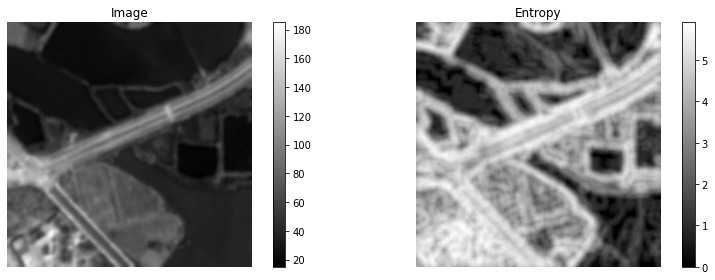
\includegraphics[width=8cm]{images/entropy.png}
\caption{Gray scale image and corresponding entropy-based image}
\end{figure}

%-------------------------------------------------------------------------
\subsection{Train and Test}

Three different settings for the ANFIS training were tried in the experiment. Since it is a Neural Network with an offline batch learning, it is quite slow in the training. What must be tried in this phase is above all to understand what is the optimal number of fuzzy sets for ANFIS. This parameter must be chosen, it is not a system output.

Three such experiments have been done. The training was done by selecting 2 fuzzy sets as parameters, then 3 and finally 4. Furthermore, all three experiments were conducted by choosing to train the ANFIS with 20 epochs and 32 of batch size.
As fuzzy sets grow, the number of fuzzy rules grows. Having $n$ variables and $m$ fuzzy sets, the number of rules will be equal to $n^{m}$. For this reason, in the three configurations there are respectively 16, 64 and 256 rules.

As the complexity of the system increases, so does the time needed to train the neuro fuzzy network. In the following table the training time for the three experiments is shown.

\begin{table}[h!]
\centering
\begin{tabular}{||c c||} 
 \hline
 Fuzzy Sets & Time \\ [0.5ex] 
 \hline\hline
 2 & 12m29s \\ 
 3 & 18m26s \\
 4 & 26m48s \\  [1ex] 
 \hline
\end{tabular}
\caption{Training time for each setting}
\label{table:2}
\end{table}

In the experiments a k-fold cross validation is used, with a train/test split of the dataset of 70/30\%. In the three configurations the overall accuracy of the system is improved as the number of fuzzy sets increases, as shown in the following table. 
\begin{table}[h!]
\centering
\begin{tabular}{||c c||} 
 \hline
 Fuzzy Sets & Accuracy \\ [0.5ex] 
 \hline\hline
 2 & 75.01\% \\ 
 3 & 76.42\% \\
 4 & 77.18\% \\  [1ex] 
 \hline
\end{tabular}
\caption{Overall accuracy for each setting}
\label{table:2}
\end{table}

Since the three configurations have a similar accuracy, and considering the complexity and the training time for the configurations with three and four fuzzy sets, in this document only the training result of the first model will be described in detail.

First of all, in the following image, the shown graph indicates the decrease of the Loss value on both the training and validation data with respect to the epochs.
\begin{figure}[h]
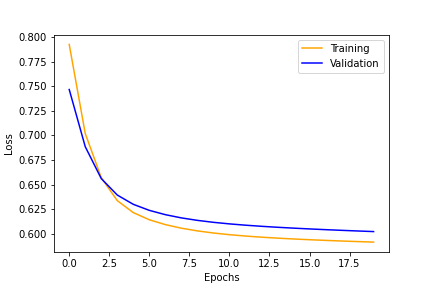
\includegraphics[width=8cm]{images/Fold_0_Val_loss.png}
\caption{Loss value for both training and validation data.}
\end{figure}

As described in the description of the model, the first layer has the task of fuzzifying the variables by assigning them membership functions. Having set two fuzzy sets for each variable (which in our case are four), the output of this layer will be two membership functions for each variable. In the following table there are the values of the computed functions, where the variables $x_0$, $x_1$, $x_2$, $x_3$ are in the order the value of the red, green and blue channels and the entropy for a certain pixel.

\begin{table}[h!]
\centering
\caption{Membership functions for each variable.}
\begin{tabular}{lclcl}
\hline
\multicolumn{1}{|l|}{Membership function}   & \multicolumn{4}{c|}{Variable}                             \\ \hline
\multicolumn{1}{|l|}{}                      & \multicolumn{2}{c|}{\mu}     & \multicolumn{2}{c|}{\sigma}  \\ \hline
\multicolumn{1}{|l|}{}                      & \multicolumn{4}{c|}{Variable $x_0$}                          \\ \hline
\multicolumn{1}{|l|}{Membership Function 1} & \multicolumn{2}{c|}{-59.26} & \multicolumn{2}{c|}{64.49}  \\ \hline
\multicolumn{1}{|l|}{Membership Function 2} & \multicolumn{2}{c|}{232.15} & \multicolumn{2}{c|}{125.59} \\ \hline
\multicolumn{1}{|l|}{}                      & \multicolumn{4}{c|}{Variable $x_1$}                          \\ \hline
\multicolumn{1}{|l|}{Membership Function 1} & \multicolumn{2}{c|}{-56.74} & \multicolumn{2}{c|}{53.36}  \\ \hline
\multicolumn{1}{|l|}{Membership Function 2} & \multicolumn{2}{c|}{233.35} & \multicolumn{2}{c|}{119.37} \\ \hline
\multicolumn{1}{|l|}{}                      & \multicolumn{4}{c|}{Variable $x_2$}                          \\ \hline
\multicolumn{1}{|l|}{Membership Function 1} & \multicolumn{2}{c|}{-54.07} & \multicolumn{2}{c|}{67.67}  \\ \hline
\multicolumn{1}{|l|}{Membership Function 2} & \multicolumn{2}{c|}{240.75} & \multicolumn{2}{c|}{127.28} \\ \hline
\multicolumn{1}{|l|}{}                      & \multicolumn{4}{c|}{Variable $x_3$}                          \\ \hline
\multicolumn{1}{|l|}{Membership Function 1} & \multicolumn{2}{c|}{-1.73}  & \multicolumn{2}{c|}{3.06}   \\ \hline
\multicolumn{1}{|l|}{Membership Function 2} & \multicolumn{2}{c|}{4.72}   & \multicolumn{2}{c|}{1.44}   \\ \hline
                                            & \multicolumn{1}{l}{}   &    & \multicolumn{1}{l}{}    &  
\end{tabular}
\end{table}
Based on these values, layers 3 and 4 of the network generated the following fuzzy rules. The the sixteen rules generated by the inference system are shown below, where $x_0$, $x_1$, $x_2$, $x_3$ are the input variables and mf1, mf2 are the related Membership Functions.
\begin{itemize}
    \item IF $x_0$ is mf1 and $x_1$ is mf1 and $x_2$ is mf1 and $x_3$ is mf1 THEN [[0.10], [0.0], [1.0], [0.98]]
    \item IF $x_0$ is mf1 and $x_1$ is mf1 and $x_2$ is mf1 and $x_3$ is mf2 THEN [[0.74], [0.61], [0.0], [1.0]]
    \item IF $x_0$ is mf1 and $x_1$ is mf1 and $x_2$ is mf2 and $x_3$ is mf1 THEN [[0.69], [1.0], [0.0], [0.68]]
    \item IF $x_0$ is mf1 and $x_1$ is mf1 and $x_2$ is mf2 and $x_3$ is mf2 THEN [[0.62], [1.0], [0.23], [0.0]]
    \item IF $x_0$ is mf1 and $x_1$ is mf1 and $x_2$ is mf1 and $x_3$ is mf1THEN [[0.0], [0.52], [1.0], [0.88]]
    \item IF $x_0$ is mf1 and $x_1$ is mf2 and $x_2$ is mf1 and $x_3$ is mf2 THEN [[0.0], [0.45], [1.0], [0.91]]
    \item IF $x_0$ is mf1 and $x_1$ is mf2 and $x_2$ is mf2 and $x_3$ is mf1 THEN [[0.60], [1.0], [0.0], [0.96]]
    \item IF $x_0$ is mf1 and $x_1$ is mf2 and $x_2$ is mf2 and $x_3$ is mf2 THEN [[1.0], [0.11], [0.0], [0.19]]
    \item IF $x_0$ is mf2 and $x_1$ is mf1 and $x_2$ is mf1 and $x_3$ is mf1 THEN [[0.99], [0.59], [1.0], [0.0]]
    \item IF $x_0$ is mf2 and $x_1$ is mf1 and $x_2$ is mf1 and $x_3$ is mf2 THEN [[0.99], [0.42], [0.37], [0.0]]
    \item IF $x_0$ is mf2 and $x_1$ is mf1 and $x_2$ is mf2 and $x_3$ is mf1 THEN [[1.0], [0.88], [0.0], [0.32]]
    \item IF $x_0$ is mf2 and $x_1$ is mf1 and $x_2$ is mf2 and $x_3$ is mf2 THEN [[1.0], [0.65], [0.42], [0.0]]
    \item IF $x_0$ is mf2 and $x_1$ is mf2 and $x_2$ is mf1 and $x_3$ is mf1 THEN [[0.0], [0.19], [0.91], [1.0]]
    \item IF $x_0$ is mf2 and $x_1$ is mf2 and $x_2$ is mf1 and $x_3$ is mf2 THEN [[0.0], [0.26], [0.45], [1.0]]
    \item IF $x_0$ is mf2 and $x_1$ is mf2 and $x_2$ is mf2 and $x_3$ is mf1 THEN [[0.0], [0.99], [0.75], [0.22]]
    \item IF $x_0$ is mf2 and $x_1$ is mf2 and $x_2$ is mf2 and $x_3$ is mf2 THEN [[1.0], [0.92], [0.84], [0.0]]
\end{itemize}

Based on this rules, the last layer classify the pixels. The test of the system gives the following scores.
\begin{table}[]
\centering
\caption{Test scores.}
\begin{tabular}{|l|l|l|l|}
\hline
\textbf{Label}              & \textbf{precision} & \textbf{recall} & \textbf{f1-score} \\ \hline
\textit{Building}           & 0.75               & 0.62            & 0.68              \\ \hline
\textit{Road}               & 0.51               & 0.52            & 0.51              \\ \hline
\textit{Vegetation}         & 0.79               & 0.88            & 0.83              \\ \hline
\textit{Water}              & 0.89               & 0.77            & 0.83              \\ \hline
                            &                    &                 &                   \\ \hline
{\ul \textbf{accuracy}}     &                    &                 & 0.75              \\ \hline
{\ul \textbf{macro avg}}    & 0.74               & 0.70            & 0.71              \\ \hline
{\ul \textbf{weighted avg}} & 0.75               & 0.75            & 0.75              \\ \hline
\end{tabular}
\end{table}

As can be seen from the test metrics, the system classifies the pixels belonging to the \textit{Water} and \textit{Vegetation} classes with good accuracy, and less those belongs to the \textit{Building} and \textit{Road} classes. To test the system and verify its effective functioning, three images were segmented, which were chosen to highlight the classification problems that emerged from the metrics.

\begin{figure}[h]
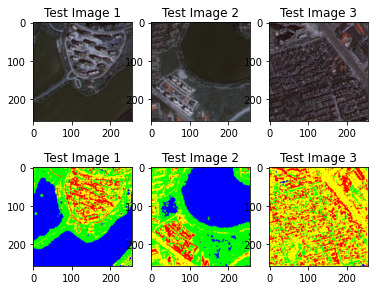
\includegraphics[width=8cm]{images/image.jpg}
\caption{New images and corresponding segmentation.}
\end{figure}

The situation depicted in the photos demonstrates what the metrics have previously suggested to us: it is possible to notice above all in the first two images how the areas relating to the Water and Vegetation classes are classified with good accuracy, while those in which Roads and Buildings are present are more confused. This is especially visible in the third photo, which frames an area with almost exclusively Builds and Roads.

%------------------------------------------------------------------------
\section{Conclusions and Future Work}

The segmentation of the test images showed that the model classifies satellite images with decent results based only on the values of the RGB values and the entropy, extracted during the pre-processing phase. Certainly RGB images are easier to find for free on internet than multispectral images, but they are not very clear. The colors in the photos are subject to variation based on the weather conditions that are present when the photo is taken, and this certainly affects the training of the system as well.

To have a better classification, it will be possible to use multispectral remotely sensed images and also, to perform texture extraction using the appropriate Gabor filters instead of entropy.
This filter allows to extract textures more efficiently, but requires a thorough study in choosing the super-parameters (i.e. frequencies and orientations).

Although this type of approach guarantees an acceptable level of accuracy and explicability, the system was slow to train compared to the more used deep learning approaches, which have the advantage of being able to use Transfer Learning and are more effective in segmentation since they are able to extract spatial features from images as well.
%-------------------------------------------------------------------------

%------------------------------------------------------------------------

{\small
\bibliographystyle{ieee_fullname}
\bibliography{egbib}
}

\end{document}
